\documentclass[12pt]{article}

\usepackage[a4paper, left=3.17cm, right=3.17cm, top=2.54cm, bottom=2.54cm]{geometry}

\usepackage[english]{babel}
\usepackage{textcmds}

\usepackage{amsthm} % for the proof-environment
\usepackage{amsmath}
\usepackage{amssymb}
\usepackage{mathtools}
\usepackage[scr=rsfs]{mathalpha}

\usepackage{xifthen}
\usepackage{caption}
\usepackage{subcaption}
\usepackage{sidecap}
\usepackage{graphicx}
\usepackage[export]{adjustbox}
\usepackage{float}
\usepackage{titlesec}
\usepackage{tikz}
\usetikzlibrary{positioning, quotes}

\usepackage{color}
\usepackage{hyperref} %clickable table of contents
\hypersetup{
    colorlinks=false, %set true if you want colored links
    linktoc=all,     %set to all if you want both sections and subsections linked
    linkcolor=blue,  %choose some color if you want links to stand out
}

\usepackage{csquotes}
\usepackage[backend=biber,style=numeric]{biblatex}
\addbibresource{references.bib}

\newcommand{\C}{\mathbb{C}}
\newcommand{\R}{\mathbb{R}}
\newcommand{\N}{\mathbb{N}}
\newcommand{\Z}{\mathbb{Z}}
\DeclarePairedDelimiter{\norm}{\lVert}{\rVert}

\renewcommand{\abstractname}{Abstract}
\titleformat{\section}
{\normalfont\large\bfseries}{\thesection}{1em}{}

\title{Structure Recognition with Graph Neural Networks \\[1em] \large Final Report for the Lab-Course Advanced Projects in Computational Physics 2}
\author{Benedikt Wenzel}
\date{\today}

\begin{document}
\maketitle

\begin{abstract}
The project lies at the intersection of Machine Learning and solid-state physics. 
A common task in solid-state physics is the classification of atomic structures, such as those found in crystals.
Machine Learning, on the other hand, is well-known for its ability to handle classification tasks. Combining these two worlds provides a powerful tool for 
classifying different crystal structures. 
As crystal structures are described by the so-called Bravais lattices, which closely relate to graphs, we will need machine learning tools capable of properly handling graph-like data.
Fortunately, in the last few years, a new type of neural networks, exactly designed for this kind of data, emerged: Graph-Neural-Networks.
The overall goal of this project is to get familiar with GNNs and apply them to classification tasks of Bravais lattices.
The code for this project is available at \url{https://github.com/BenWen0/ComputationalPhysics2}.
\end{abstract}

\tableofcontents
\newpage

\section{Background}
This introductory section lays the theoretical foundation of Bravais lattices and GNNs. 
We start with a short recap of lattice structures in 2d and 3d and then continue with 
the most fundamental background of Graph-Neural Networks (GNN). 
Results on Bravais lattices can be found in many textbooks. Subsection~\ref{sec:brav_latt} follows~\cite{Schwarzenberger} and ~\cite{symGroupsApplications}.
Introduction to Graph Neural Networks can be found for example in~\cite{IntroMessagePassing} which is also the main reference for section~\ref{sec:fund_gnns}.

\subsection{Bravais lattice}
\label{sec:brav_latt}
Let $d\in\N$ and $\{b_i\}_{i=1,\dots,d}\subset \R^d$ a basis of $\R^d$. The set 
\begin{equation*}
    \Omega\coloneq\left\{\sum_{i=1}^{d}z_i b_i: z_i\in\Z\,\forall i\in\{1,\dots,d\}\right\}
\end{equation*}
is called a $d$-dimensional lattice. Given any subset $S\subset\R^d$, we define its point group $G_S$ to be
\begin{equation*}
    G_S\coloneq \left\{M\in O(d) : MS=S\right\}\subset O(d).
\end{equation*}
$G_S$ is obviously a subgroup of $O(d)$. We say that two $d$-dimensional lattices $\Omega_1, \Omega_2\subset \R^d$ are of the same Bravais type if
there exists $g\in GL_n(\R)$ such that $G_{\Omega_1}=g G_{\Omega_2} g^{-1}$ and $\Omega_1=g\Omega_2$. 
Being of the same Bravais type introduces an equivalence relation on the set of all $d$-dimensional lattices. We refer to the equivalence classes as Bravais classes.
A natural question arising is about the total number of Bravais classes. Despite being a very interesting and challenging problem,
we will leave this question to the mathematicians. For us, the result is more important than the actual proof. One obtains the following result:
For $d=2$ there are 5 Bravais classes and for $d=3$ there are 14 Bravais classes. 
\begin{figure}[b]
    \centering
    \begin{subfigure}[t]{0.3\textwidth}
        \centering
        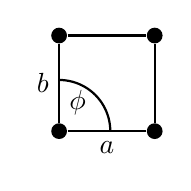
\begin{tikzpicture}[
            node distance=1cm and 1cm,
            node/.style={circle, inner sep=0pt, fill=black, minimum size=2mm}
        ]
        \node[node] (n1) {};
        \node[node] (n2) [above=of n1]{}; 
        \node[node] (n3) [right=of n1]{};  
        \node[node] (n4) [right=of n2]{}; 
        \draw[-, thick]  (n1) -- node[anchor=east, black]{$b$} (n2);   
        \draw[-, thick]  (n1) -- node[anchor=north, black]{$a$} (n3); 
        \draw[-, thick]  (n2) -- (n4);
        \draw[-, thick]  (n4) -- (n3);        
        \draw [black,thick,domain=0:90] plot ({0.65*cos(\x)}, {0.65*sin(\x)}) node[anchor=north west, black]{$\phi$};
        \end{tikzpicture}
        \caption{$\phi=\frac{\pi}{2}$, $a=b$}
    \end{subfigure}
    \hfill
    \begin{subfigure}[t]{0.3\textwidth}
        \centering
        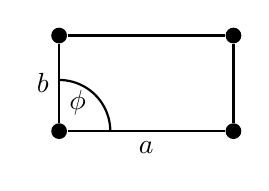
\begin{tikzpicture}[
            node distance=1cm and 2cm,
            node/.style={circle, inner sep=0pt, fill=black, minimum size=2mm}
        ]
        \node[node] (n1) {};
        \node[node] (n2) [above=of n1]{}; 
        \node[node] (n3) [right=of n1]{};  
        \node[node] (n4) [right=of n2]{}; 
        \draw[-, thick]  (n1) -- node[anchor=east, black]{$b$} (n2);   
        \draw[-, thick]  (n1) -- node[anchor=north, black]{$a$} (n3); 
        \draw[-, thick]  (n2) -- (n4);
        \draw[-, thick]  (n4) -- (n3);        
        \draw [black,thick,domain=0:90] plot ({0.65*cos(\x)}, {0.65*sin(\x)}) node[anchor=north west, black]{$\phi$};
        \end{tikzpicture}
        \caption{$\phi=\frac{\pi}{2}$, $a\neq b$}
    \end{subfigure}
    \hfill
    \begin{subfigure}[t]{0.3\textwidth}
        \centering
        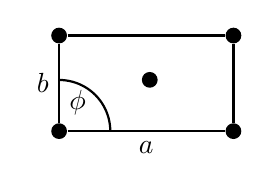
\begin{tikzpicture}[
            node distance=1cm and 2cm,
            node/.style={circle, inner sep=0pt, fill=black, minimum size=2mm}
        ]
        \node[node] (n1) {};
        \node[node] (n2) [above=of n1]{}; 
        \node[node] (n3) [right=of n1]{};  
        \node[node] (n4) [right=of n2]{}; 
        \node[node] (n5) [above right=0.5cm and 1cm of n1] {};
        \draw[-, thick]  (n1) -- node[anchor=east, black]{$b$} (n2);   
        \draw[-, thick]  (n1) -- node[anchor=north, black]{$a$} (n3); 
        \draw[-, thick]  (n2) -- (n4);
        \draw[-, thick]  (n4) -- (n3);        
        \draw [black,thick,domain=0:90] plot ({0.65*cos(\x)}, {0.65*sin(\x)}) node[anchor=north west, black]{$\phi$};
        \end{tikzpicture}
        \caption{$\phi=\frac{\pi}{2}$, $a\neq b$}
    \end{subfigure}

    \begin{subfigure}[t]{0.3\textwidth}
        \centering
        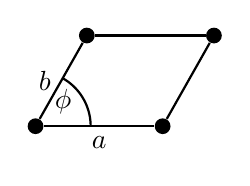
\begin{tikzpicture}[
            node distance=1.2cm and 1.4cm,
            node/.style={circle, inner sep=0pt, fill=black, minimum size=2mm}
        ]
        \node[node] (n1) {};
        \node[node] (n2) [above right=1cm and 0.5cm of n1]{}; 
        \node[node] (n3) [right=of n1]{};  
        \node[node] (n4) [right=of n2]{}; 
        \draw[-, thick]  (n1) -- node[anchor=east, black]{$b$} (n2);   
        \draw[-, thick]  (n1) -- node[anchor=north, black]{$a$} (n3); 
        \draw[-, thick]  (n2) -- (n4);
        \draw[-, thick]  (n4) -- (n3);        
        \draw [black,thick,domain=0:60] plot ({0.7*cos(\x)}, {0.7*sin(\x)}) node[anchor=north, black]{$\phi$};
        \end{tikzpicture}
        \caption{$\phi\neq\frac{\pi}{2}$, $a\neq b$}
    \end{subfigure}
    \begin{subfigure}[t]{0.3\textwidth}
        \centering
        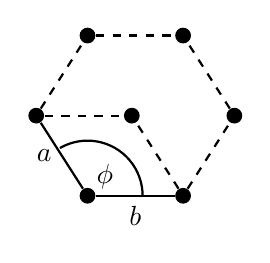
\begin{tikzpicture}[
            node distance=1cm and 1cm,
            node/.style={circle, inner sep=0pt, fill=black, minimum size=2mm}
        ]
        \node[node,label={[label distance=-0.15cm]80:$\phi$}] (n1) {};
        \node[node] (n2) [right=of n1]{}; 
        \node[node] (n3) [above left=0.866cm and 0.5cm of n1]{};
        \node[node] (n4) [above left=0.866cm and 0.5cm of n2]{};  
        \node[node] (n5) [above right=0.866cm and 0.5cm of n2]{};
        \node[node] (n6) [above right=0.866cm and 0.5cm of n3]{};
        \node[node] (n7) [above left=0.866cm and 0.5cm of n5]{};
        \draw[-, thick]  (n1) -- node[anchor=north, black]{$b$} (n2);   
        \draw[-, thick]  (n1) -- node[anchor=east, black]{$a$} (n3); 
        \draw[dashed, thick]  (n2) -- (n4);
        \draw[dashed, thick]  (n2) -- (n5); 
        \draw[dashed, thick]  (n3) -- (n4);
        \draw[dashed, thick]  (n3) -- (n6);
        \draw[dashed, thick]  (n5) -- (n7);
        \draw[dashed, thick]  (n6) -- (n7);
        \draw [black,thick,domain=0:120] plot ({0.7*cos(\x)}, {0.7*sin(\x)});
        \end{tikzpicture}
        \caption{$\phi=\frac{2\pi}{3}$, $a=b$}
    \end{subfigure}
    
    \caption{All different Bravais classes in two dimensions. They are called (a) square, (b) rectangle,
    (c) centered rectangle, (d) oblique, (e) hexagonal.}
    \label{fig:bravais2D}
\end{figure}
Roughly speaking, they can be distinguished by the relative lengths of the basis vectors $b_i$ and the angles between them.
Visualizations of all Bravais classes for $d=2$ can be found in figure~\ref{fig:bravais2D}.
Visualizations for $d=3$ and further notes on each Bravais class can be found for example in~\cite{kittel}.


\subsection{Introduction to Neural Networks}
\label{sec:intro_nn}
Stating a precise definition of \glqq{}Neural Network\grqq{} is quite involved. 
Hence, we will only speak about the most fundamental type of neural networks, the so-called feed forward neural networks. 
Even for these simple networks, a precise definition is rather lengthy. We have to introduce some notation first:
Let $l\in\N_{\geq2}$, $n_0,n_1\dots,n_l\in\N$ and for each $i\in\N, i\leq l$ 
choose an affine linear map $T^{(i)}:\R^{n_{i-1}}\to\R^{n_i}$ and a smooth map $a^{(i)}:\R\to\R$.
Denoting with $f^{(i)}:\R^{n_i}\to\R^{n_i}$ the function acting element wise by $a^{(i)}$ (i.e $f^{(i)}(x_1, \dots, x_{n_i})=(a^{(i)}(x_1),\dots, a^{(i)}(x_{n_i}))$), 
we define the composition 
\begin{equation*} 
\tilde{F}\coloneq T^{(l)}\circ f^{(l-1)}\circ T^{(l-1)}\circ\dots\circ f^{(2)}\circ T^{(2)}\circ f^{(1)}\circ T^{(1)}:\R^{n_0}\to\R^{n_l}.
\end{equation*}
Recall that for any affine linear map $L:\R^n\to\R^m$ there exist $b\in\R^m$ and $W\in \text{Mat}(n\times m,\R)$ such that 
$Lx=W^Tx+b$ for all $x\in\R^n$ (the transposition is just for our convenience later on). Hence, to each $T^{(i)}$ corresponds a matrix $W^{(i)}\in\text{Mat}(n_{i-1}\times n_i,\R)$ called the weight-matrix and a vector
$b^{(i)}\in\R^{n_i}$ called bias such that $T^{(i)}x=\left(W^{(i)}\right)^Tx + b^{(i)}$.
We introduce further notation: Obviously, we can think of $W^{(i)}$ as an element in $\R^{n_{i-1}n_i}$. 
Let $\theta=(W^{(1)},b^{(1)},\dots,W^{(l)},b^{(l)})\in\R^{n_0n_1}\times\R^{n_1}\times\dots\times\R^{n_{l-1}n_l}\times\R^{l}$. 
Clearly, $\tilde{F}$ depends on the choice of $T^{(l)}$ and hence on the choice of $\theta$. 
Correspondingly, for each such $\theta$ we can build a map $\tilde{F}=F_\theta$.
With this notation in mind, we are ready to define what a neural network should be: The map
\begin{equation*}
    F:\R^{n_0n_1}\times\R^{n_1}\times\dots\times\R^{n_{l-1}n_l}\times\R^{n_l}\to C(\R^{n_0},\R^{n_l}), \quad\theta\mapsto F_\theta
\end{equation*}
is called (feed forward) neural network with $l$ layers and activation function $a^{(i)}$ in layer $i$.

Though this definition might seem technical, it bears a visual explanation:
It is best explained with figure~\ref{fig:nn}. We can view $F_\theta:\R^{n_0}\to\R^{n_l}$ as a graph-like structure. Each coordinate $x_i$ 
of an input vector $x\in\R^{n_0}$ can be thought of as a node. Applying $f^{(1)}\circ T^{(1)}$ to $x$ yields a
new vector $y^1=f^{(1)}\circ T^{(1)}(x)\in\R^{n_1}$. The coordinates of $y^1$ can again be interpreted as nodes. All these nodes (coordinates) together constitute the new layer
of the network. Applying $f^{(2)}\circ T^{(2)}$ to $y^1$ yields a new layer $y^2$ and so on. The last layer $y^l$ is then given by $F_\theta(x)$.
Going from layer $i-1$ to the layer $i$ can be visualized as follows: 
According to the above definitions we have
\begin{align*}
    y^{i}_j&=a^{(i)}\left(T^{(i)}\left(y^{i-1}\right)\right)_j\\
    &=a^{(i)}\left(\sum_{k=1}^{n_{i-1}}\left(W^{(i)}\right)^T_{jk}y^{i-1}_k+b^{(i)}_j\right)\\
    &=a^{(i)}\left(\sum_{k=1}^{n_{i-1}}W^{(i)}_{kj}y^{i-1}_k+b^{(i)}_j\right).
\end{align*}
Up to application of $a^{(i)}$, the node $y^i_j$ is a weighted sum of all nodes $y^{i-1}_k$ in the previous layer (in addition to a constant bias value $b^{(i)}_j$).
The matrix element $W^{(i)}_{kj}$ describes how much the node $y^i_j$ is influenced by node $y^{i-1}_k$. 
We picture an edge from node $y^{i-1}_k$ to node $y^i_j$ which has the weight $W^{(i)}_{kj}$. Consequently, the matrix $W^{(i)}$ is called weight-matrix.
\begin{figure}[h]
    \centering
    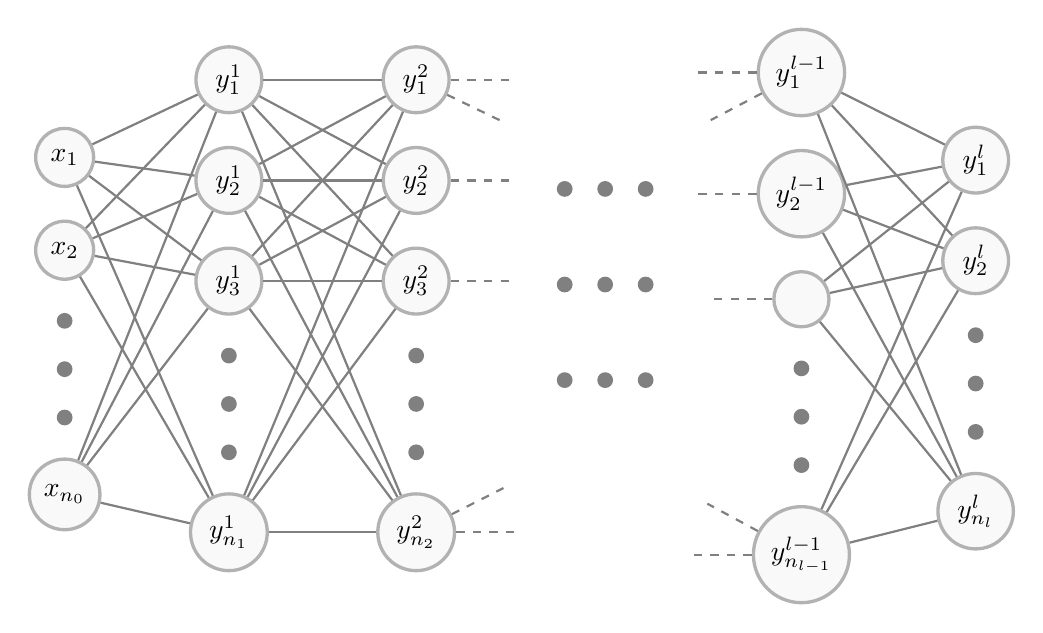
\begin{tikzpicture}[
        node distance=0.4cm and 1.5cm,
        node/.style={circle, draw=gray!60, fill=gray!5, very thick, minimum size=7mm},
        node_missing/.style={circle, inner sep=0pt, fill=gray, minimum size=2mm},
        node_invisible/.style={circle, inner sep=0pt, fill=red, minimum size=0mm}
        ]

        %Nodes input layer
        \node[node] (1_1) {$x_1$};
        \node[node] (1_2) [below=of 1_1] {$x_2$};
        \node[node_missing] (m_1_1) [below=of 1_2] {};
        \node[node_missing] (m_1_2) [below=of m_1_1] {};
        \node[node_missing] (m_1_3) [below=of m_1_2] {};
        \node[node] (1_3) [below=of m_1_3] {$x_{n_0}$};

        %Nodes hidden layer 1
        \node[node] (2_1) [above right=of 1_1] {$y^1_1$};
        \node[node] (2_2) [below=of 2_1] {$y^1_2$};
        \node[node] (2_3) [below=of 2_2] {$y^1_3$};
        \node[node_missing] (m_2_1) [below=of 2_3] {};
        \node[node_missing] (m_2_2) [below=of m_2_1] {};
        \node[node_missing] (m_2_3) [below=of m_2_2] {};
        \node[node] (2_4) [below=of m_2_3] {$y^1_{n_1}$};

        %Nodes hidden layer 2
        \node[node] (3_1) [right=of 2_1] {$y^2_1$};
        \node[node] (3_2) [below=of 3_1] {$y^2_2$};
        \node[node] (3_3) [below=of 3_2] {$y^2_3$};
        \node[node_missing] (m_3_1) [below=of 3_3] {};
        \node[node_missing] (m_3_2) [below=of m_3_1] {};
        \node[node_missing] (m_3_3) [below=of m_3_2] {};
        \node[node] (3_4) [below=of m_3_3] {$y^2_{n_2}$};

        %missing hidden layers
        \node[node_missing] (m_4_1) [below right=1cm and 1.5cm of 3_1] {};
        \node[node_missing] (m_4_2) [below=1cm of m_4_1] {};
        \node[node_missing] (m_4_3) [below=1cm of m_4_2] {};
        \node[node_missing] (m_5_1) [right=0.3cm of m_4_1] {};
        \node[node_missing] (m_5_2) [below=1cm of m_5_1] {};
        \node[node_missing] (m_5_3) [below=1cm of m_5_2] {};
        \node[node_missing] (m_6_1) [right=0.3cm of m_5_1] {};
        \node[node_missing] (m_6_2) [below=1cm of m_6_1] {};
        \node[node_missing] (m_6_3) [below=1cm of m_6_2] {};
        
        %Nodes hidden layer 3
        \node[node] (7_1) [above right=1cm and 1.5cm of m_6_1] {$y^{l-1}_1$};
        \node[node] (7_2) [below=of 7_1] {$y^{l-1}_2$};
        \node[node] (7_3) [below=of 7_2] {};
        \node[node_missing] (m_7_1) [below=of 7_3] {};
        \node[node_missing] (m_7_2) [below=of m_7_1] {};
        \node[node_missing] (m_7_3) [below=of m_7_2] {};
        \node[node] (7_4) [below=of m_7_3] {$y^{l-1}_{n_{l-1}}$};

        %Nodes output layer
        \node[node] (8_1) [below right=of 7_1] {$y^{l}_1$};
        \node[node] (8_2) [below=of 8_1] {$y^{l}_2$};
        \node[node_missing] (m_8_1) [below=of 8_2] {};
        \node[node_missing] (m_8_2) [below=of m_8_1] {};
        \node[node_missing] (m_8_3) [below=of m_8_2] {};
        \node[node] (8_3) [below=of m_8_3] {$y^{l}_{n_l}$};

        %invisible nodes
        \node[node_invisible] (inv_1_1) [right=0.75cm of 3_1] {};
        \node[node_invisible] (inv_1_2) [below right=0.2cm and 0.75cm of 3_1] {};
        \node[node_invisible] (inv_1_3) [above right=0.2cm and 0.75cm of 3_4] {};
        \node[node_invisible] (inv_1_4) [right=0.75cm of 3_4] {};
        \node[node_invisible] (inv_1_5) [right=0.75cm of 3_2] {};
        \node[node_invisible] (inv_1_6) [right=0.75cm of 3_3] {};
        \node[node_invisible] (inv_2_1) [left=0.75cm of 7_1] {};
        \node[node_invisible] (inv_2_2) [below left=0.2cm and 0.75cm of 7_1] {};
        \node[node_invisible] (inv_2_3) [above left=0.2cm and 0.75cm of 7_4] {};
        \node[node_invisible] (inv_2_4) [left=0.75cm of 7_4] {};
        \node[node_invisible] (inv_2_5) [left=0.75cm of 7_2] {};
        \node[node_invisible] (inv_2_6) [left=0.75cm of 7_3] {};
        %connections with invisible nodes
        \draw[dashed, thick, gray]  (3_1) -- (inv_1_1);
        \draw[dashed, thick, gray]  (3_1) -- (inv_1_2);
        \draw[dashed, thick, gray]  (3_2) -- (inv_1_5);
        \draw[dashed, thick, gray]  (3_3) -- (inv_1_6);
        \draw[dashed, thick, gray]  (3_4) -- (inv_1_3);
        \draw[dashed, thick, gray]  (3_4) -- (inv_1_4);
        \draw[dashed, thick, gray]  (7_1) -- (inv_2_1);
        \draw[dashed, thick, gray]  (7_1) -- (inv_2_2);
        \draw[dashed, thick, gray]  (7_2) -- (inv_2_5);
        \draw[dashed, thick, gray]  (7_3) -- (inv_2_6);
        \draw[dashed, thick, gray]  (7_4) -- (inv_2_3);
        \draw[dashed, thick, gray]  (7_4) -- (inv_2_4);

        %connections input and first hidden layer
        \draw[-, thick, gray]  (1_1) -- (2_1);
        \draw[-, thick, gray]  (1_1) -- (2_2);
        \draw[-, thick, gray]  (1_1) -- (2_3);
        \draw[-, thick, gray]  (1_1) -- (2_4);
        \draw[-, thick, gray]  (1_2) -- (2_1);
        \draw[-, thick, gray]  (1_2) -- (2_2);
        \draw[-, thick, gray]  (1_2) -- (2_3);
        \draw[-, thick, gray]  (1_2) -- (2_4);
        \draw[-, thick, gray]  (1_3) -- (2_1);
        \draw[-, thick, gray]  (1_3) -- (2_2);
        \draw[-, thick, gray]  (1_3) -- (2_3);
        \draw[-, thick, gray]  (1_3) -- (2_4);

        %connections first and second hidden layer
        \draw[-, thick, gray]  (2_1) -- (3_1);
        \draw[-, thick, gray]  (2_1) -- (3_2);
        \draw[-, thick, gray]  (2_1) -- (3_3);
        \draw[-, thick, gray]  (2_1) -- (3_4);
        \draw[-, thick, gray]  (2_2) -- (3_1);
        \draw[-, thick, gray]  (2_2) -- (3_2);
        \draw[-, thick, gray]  (2_2) -- (3_3);
        \draw[-, thick, gray]  (2_2) -- (3_4);
        \draw[-, thick, gray]  (2_3) -- (3_1);
        \draw[-, thick, gray]  (2_3) -- (3_2);
        \draw[-, thick, gray]  (2_3) -- (3_3);
        \draw[-, thick, gray]  (2_3) -- (3_4);
        \draw[-, thick, gray]  (2_4) -- (3_1);
        \draw[-, thick, gray]  (2_4) -- (3_2);
        \draw[-, thick, gray]  (2_4) -- (3_3);
        \draw[-, thick, gray]  (2_4) -- (3_4);

        %connections output and last hidden layer
        \draw[-, thick, gray]  (7_1) -- (8_1);
        \draw[-, thick, gray]  (7_1) -- (8_2);
        \draw[-, thick, gray]  (7_1) -- (8_3);
        \draw[-, thick, gray]  (7_2) -- (8_1);
        \draw[-, thick, gray]  (7_2) -- (8_2);
        \draw[-, thick, gray]  (7_2) -- (8_3);
        \draw[-, thick, gray]  (7_3) -- (8_1);
        \draw[-, thick, gray]  (7_3) -- (8_2);
        \draw[-, thick, gray]  (7_3) -- (8_3);
        \draw[-, thick, gray]  (7_4) -- (8_1);
        \draw[-, thick, gray]  (7_4) -- (8_2);
        \draw[-, thick, gray]  (7_4) -- (8_3);
    \end{tikzpicture}
    \caption{Visualization of a feed forward neural network.}
    \label{fig:nn}
\end{figure}

With the visuals in mind, we can explain what neural networks are used for and how they are being used. 
The purpose of neural networks lies in the  approximation of unknown functions. 
Suppose we were given a function $G:\R^n\to\R^m$ from which we only know values at $D$-many ($D\in\N$) points $x_1,\dots,x_D\in\R^n$, 
i.e. only the values $y_1=G(x_1),\dots,y_D=G(x_D)$ are known.
Choose $l\in\N$, set $n_0=n$, $n_l=m$ and consider the neural network
\begin{equation*}
    F:\R^{n_0n_1}\times\R^{n_1}\times\dots\times\R^{n_{l-1}n_l}\times\R^{n_l}\to C(\R^{n_0},\R^{n_l}), \quad\theta\mapsto F_\theta.
\end{equation*}
We can then try to find an \glqq{}optimal\grqq{} $\theta$ such that $F_\theta\approx G$. 
To do so, we have to introduce a measure for how much $F_\theta$ differs from $G$. 
This is commonly called a cost/loss function, i.e. a function $C:\R^m\times\R^m\to\R$, that maps to a pair $(F_\theta(x_i), y_i)$ a real value
$C(F_\theta(x_i),y_i)$ that can be interpreted as a distance between the true value $y_i$ and the predicted value $F_\theta(x_i)$.
Finding an optimal $\theta$ is achieved by minimizing the map $\theta\to C(F_\theta(x_i),y_i)$ for all $i=1,\dots,D$.
This optimization is called \glqq{}training the neural network\grqq{}. 
There is a whole branch of mathematics about these kinds of optimization of problems. 
A common way to do this is by means of the gradient descent method.
Roughly speaking, the idea is the following: Calculate the gradient of the map $\theta\mapsto C(F_\theta(x_i),y_i)$ for a fixed $i=1,\dots,D$, 
and then change $\theta$ slightly in the opposite direction of the gradient.
How much $\theta$ is changed, depends on the so-called learning rate $\eta\in\R_+$. 
As $F_\theta$ is a large composition, computing the gradient basically comes down to repeated application of the chain rule. 
An efficient algorithm that does exactly this and is widely used is called backpropagation. We can repeat this step until we found a $\theta$ such that 
$C(F\theta(x_i),y_i)$ is sufficiently small for all $i=1,\dots,d$.

Furthermore, there are many more techniques and tools (like optimizers, batching, ...) to make the training more efficient, faster converging and less time-consuming. 
However, this section was intended to give only a rough overview. Hence, we will not go into more detail. 
For additional information, there is a vast amount of literature on these topics, see for example \cite{bookNN1}, \cite{bookNN2} and \cite{paperHyperparameter}.

\subsection{Fundamentals of Graphs and Graph Neural Networks}
\label{sec:fund_gnns}
To talk about graphs, we first have to agree on some notation: Let $V$ be a set and $E\subset V\times V$. The tuple $G=(V,E)$ is called a graph. Furthermore, we call an element $x\in V$ a node and a tuple 
$(x, y)\in E$ a directed edge from $x$ to $y$. Suppose there is a directed edge from $x$ to $y$, then we say that $x$ is a neighbor of $y$. 
In case $(x,y)\in E$ implies $(y,x)\in E$, we speak of an undirected graph.
In that case, we can think of elements in $E$ as unordered tuples $\{x,y\}$ instead of ordered ones. We still call $\{x,y\}$ an edge between $x$ and $y$.
For $y\in V$ we define the neighborhood $N_y$ of $y$ to be the set of all neighbors, i.e.
\begin{equation}
    \label{eq:def_neighbors}
    N_y\coloneq\left\{x\in V : (x,y)\in E\right\}\subset V.
\end{equation}
Furthermore, we assign to each node $x\in V$ a vector $v_x\in\R^n$ called node feature and to each edge $(x, y)\in E$ a vector $e_{x,y}\in\R^m$ called edge feature. 

Roughly, a GNN takes a graph with all its nodes and edge features as an input and manipulates these features in each step. 
More than that, a GNN can transform the structure of the graph itself, e.g. by introducing new nodes or edges. 
However, we will not go into detail about this possibility and stick to the simpler case of manipulating only node and edge-features.
Furthermore, we restrict ourselves to the case where the GNN does not alter the edge features.
\begin{SCfigure}[1][ht]
\centering
\label{fig:gnn}
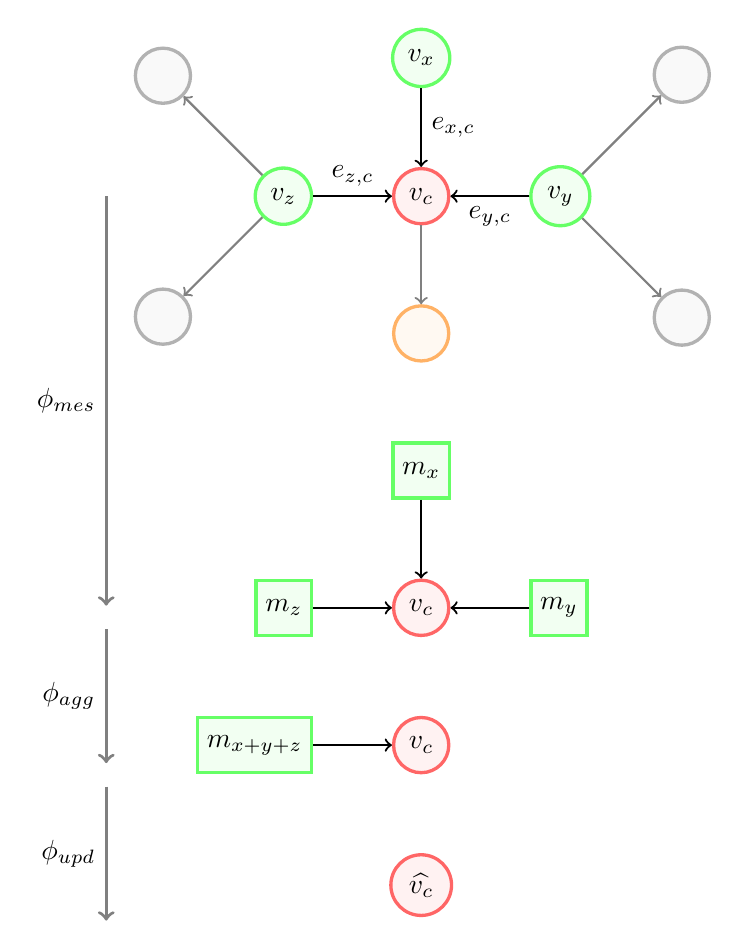
\begin{tikzpicture}[
    node_r/.style={circle, draw=red!60, fill=red!5, very thick, minimum size=7mm},
    node_o/.style={circle, draw=orange!60, fill=orange!5, very thick, minimum size=7mm},
    node_g/.style={circle, draw=gray!60, fill=gray!5, very thick, minimum size=7mm},
    node/.style={circle, draw=green!60, fill=green!5, very thick, minimum size=7mm},
    mess/.style={rectangle, draw=green!60, fill=green!5, very thick, minimum size=7mm},
    ]
    %Nodes step 1
    \node[node_r] (centernode)                          {$v_c$};
    \node[node] (top)           [above=of centernode]   {$v_x$};
    \node[node_o] (bottom)        [below=of centernode]   {};
    \node[node] (right)         [right=of centernode]   {$v_y$};
    \node[node] (left)          [left=of centernode]    {$v_z$};
    \node[node_g] (llt)           [above left=of left]    {};
    \node[node_g] (llb)           [below left=of left]    {};
    \node[node_g] (rrt)           [above right=of right]    {};
    \node[node_g] (rrb)           [below right=of right]    {};

    %Nodes step 2
    \node[mess] (mess_top)           [below=of bottom]   {$m_x$};
    \node[node_r] (centernode_2)  [below=of mess_top]     {$v_c$};
    \node[mess] (mess_right)         [right=of centernode_2]   {$m_y$};
    \node[mess] (mess_left)          [left=of centernode_2]    {$m_z$};

    %Nodes step 3
    \node[node_r] (centernode_3)  [below=of centernode_2]     {$v_c$};
    \node[mess] (mess_final)      [left=of centernode_3]   {$m_{x+y+z}$};

    %Nodes step 4
    \node[node_r] (centernode_4)  [below=of centernode_3]     {$\widehat{v_c}$};
    
    %Lines step 1
    \draw[->, thick]  (top.south) -- node[anchor=west]{$e_{x,c}$} (centernode.north);
    \draw[->, thick] (left.east) -- node[anchor=south]{$e_{z,c}$} (centernode.west);
    \draw[->, thick] (right.west) -- node[anchor=north]{$e_{y,c}$} (centernode.east);
    \draw[->, thick, gray] (centernode.south) -- (bottom.north);
    \draw[->, thick, gray] (left.north west) -- (llt.south east);
    \draw[->, thick, gray] (left.south west) -- (llb.north east);
    \draw[->, thick, gray] (right.north east) -- (rrt.south west);
    \draw[->, thick, gray] (right.south east) -- (rrb.north west);

    %Lines step 2
    \draw[->, thick]  (mess_top.south) -- (centernode_2.north);
    \draw[->, thick] (mess_left.east) -- (centernode_2.west);
    \draw[->, thick] (mess_right.west) -- (centernode_2.east);

    %Lines step 3
    \draw[->, thick]  (mess_final.east) -- (centernode_3.west);

    \draw[->, very thick, gray] (-4,-0) -- node[anchor=east, black]{$\phi_{mes}$} (-4,-5.2);
    \draw[->, very thick, gray] (-4,-5.5) -- node[anchor=east, black]{$\phi_{agg}$} (-4,-7.2);
    \draw[->, very thick, gray] (-4,-7.5) -- node[anchor=east, black]{$\phi_{upd}$} (-4,-9.2);
    %\draw[->] (rightsquare.south) .. controls +(down:7mm) and +(right:7mm) .. (lowercircle.east);
\end{tikzpicture}
\caption{Illustration of the message passing procedure according to equation~\eqref{eq:mess_pass}. 
The neighbors of node $c$ (red) are the nodes $x,y,z$ (green). Attention: According to equation~\eqref{eq:def_neighbors} the orange node is not regarded as a neighbor of $c$ as the edge points in the wrong direction.
For each neighbor ($x,y,z$), $\phi_{mes}$ computes messages ($m_x,m_y,m_z$) which are sent to $c$.
Then, $\phi_{agg}$ aggregates these three messages and outputs one overall message $m_{x+y+z}$ that is sent to $c$. 
In the last step, $\phi_{upd}$ updates the node value $v_c$ to a new value $\widehat{v_c}$.  
}
\end{SCfigure}
Let us make these ideas a bit more rigorous (see figure~\ref{fig:gnn} for an illustration):  
Let $(V,E)$ be a graph with node features $\{v_x\in\R^n : x\in V\}$ and edge features $\{e_{x,y}\in\R^m:(x,y)\in E\}$.
For each $c\in V$ a new node feature $\widehat{v_c}$ is calculated according to the following rule
\begin{equation}
    \label{eq:mess_pass}
    \widehat{v_c}=\phi_{upd}\left(
        v_c, \phi_{agg}\left(\left\{
            \phi_{mes}\left(v_y,v_c, e_{y,c}\right):y\in N_c
            \right\}\right)
    \right),
\end{equation}
where $\phi_{upd},\phi_{agg},\phi_{mes}$ denote differentiable functions. These three functions are commonly interpreted as follows:
$\phi_{mes}$ takes as inputs the node value $v_c$ and the node value $v_y$ of one neighbor $y$ of $c$ as well as the value $e_{y,c}$ of the edge $(y,c)$. 
Depending on these inputs, it then computes a value, which can be thought of as a message originating from node $y$ which is sent to node $c$.
$\phi_{agg}$ collects all these messages to node $c$ and aggregates them in some way, so that the output can be thought of as one overall message to node $c$.
$\phi_{upd}$ takes this overall message as well as the value of node $c$ and computes, how the value of node $c$ is altered.
Unsurprisingly, this scheme is called Message-Passing-Layer. Given a specific problem, that is required to be solved by a GNN, the challenge is to make appropriate choices
for $\phi_{upd},\phi_{agg},\phi_{mes}$ that suit the problem at hand. Furthermore, one has to decide how many iterations of the above procedure are suitable.

\subsection{Percolation}
\label{sec:intro_percolation}
\begin{columns}
    \begin{column}[t]{0.7\textwidth}
        Given are
        \begin{itemize}
            \item graph $G=(V,E)$
            \item one position $(n_x,n_y)$ inside unit square for each node $n\in V$
            \item small stripes at the edges of the unit square
        \end{itemize}
        $G$ is called percolating, if there are nodes $n,m\in V$ such that
        \begin{enumerate}
            \item there is a cycle containing $n$ and $m$
            \item $n$ and $m$ are connected by an edge
            \item $n$ and $m$ lie in opposite stripes
        \end{enumerate}
    \end{column} 
    \begin{column}[t]{0.3\textwidth}
        \vspace{-1cm}
        \begin{figure}[t]
            \centering
            %\hfill
            \begin{subfigure}{\textwidth}
                \centering
                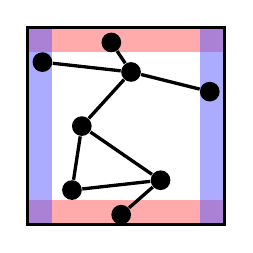
\begin{tikzpicture}[
                    node/.style={circle, inner sep=0pt, fill=black, minimum size=2.5mm}
                ]
                \useasboundingbox[fill=white](0,0) rectangle(0.625*4,0.625*4);
                \fill[red!65, fill opacity=0.5] (0,0) rectangle (0.625*4, 0.625*0.5);
                \fill[red!65, fill opacity=0.5] (0,0.625*3.5) rectangle (0.625*4, 0.625*4);
                \fill[blue!65, fill opacity=0.5] (0,0) rectangle (0.625*0.5, 0.625*4);
                \fill[blue!65, fill opacity=0.5] (0.625*3.5,0) rectangle (0.625*4, 0.625*4);
                \draw[black, very thick] (0,0) rectangle (0.625*4,0.625*4);
                \node[node] at (0.625*0.3, 0.625*3.3) (n1) {};
                \node[node] at (0.625*1.1, 0.625*2.0) (n2) {};
                \node[node] at (0.625*0.9, 0.625*0.7) (n3) {};
                \node[node] at (0.625*2.7, 0.625*0.9) (n4) {};
                \node[node] at (0.625*2.1, 0.625*3.1) (n5) {};
                \node[node] at (0.625*3.7, 0.625*2.7) (n6) {};
                \node[node] at (0.625*1.7, 0.625*3.7) (n7) {};
                \node[node] at (0.625*1.9, 0.625*0.2) (n8) {};
                \draw[very thick]  (n1) -- (n5);
                \draw[very thick]  (n5) -- (n2);
                \draw[very thick]  (n5) -- (n6);
                \draw[very thick]  (n2) -- (n4);
                \draw[very thick]  (n3) -- (n4);
                \draw[very thick]  (n2) -- (n3);
                \draw[very thick]  (n5) -- (n7);
                \draw[very thick]  (n8) -- (n4);
                \end{tikzpicture}
                \caption{non-percolating}
            \end{subfigure}
            \par\bigskip
            \begin{subfigure}{\textwidth}
                \centering
                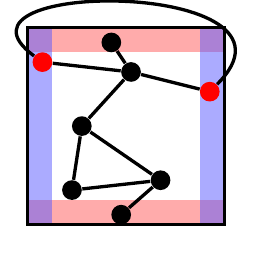
\begin{tikzpicture}[
                    node/.style={circle, inner sep=0pt, fill=black, minimum size=2.5mm},
                    node_c/.style={circle, inner sep=0pt, fill=red, minimum size=2.5mm}
                ]
                \useasboundingbox[fill=white](0,0) rectangle(0.625*4,0.625*4);
                \fill[red!65, fill opacity=0.5] (0,0) rectangle (0.625*4, 0.625*0.5);
                \fill[red!65, fill opacity=0.5] (0,0.625*3.5) rectangle (0.625*4, 0.625*4);
                \fill[blue!65, fill opacity=0.5] (0,0) rectangle (0.625*0.5, 0.625*4);
                \fill[blue!65, fill opacity=0.5] (0.625*3.5,0) rectangle (0.625*4, 0.625*4);
                \draw[black, very thick] (0,0) rectangle (0.625*4,0.625*4);
                \node[node_c] at (0.625*0.3, 0.625*3.3) (n1) {};
                \node[node] at (0.625*1.1, 0.625*2.0) (n2) {};
                \node[node] at (0.625*0.9, 0.625*0.7) (n3) {};
                \node[node] at (0.625*2.7, 0.625*0.9) (n4) {};
                \node[node] at (0.625*2.1, 0.625*3.1) (n5) {};
                \node[node_c] at (0.625*3.7, 0.625*2.7) (n6) {};
                \node[node] at (0.625*1.7, 0.625*3.7) (n7) {};
                \node[node] at (0.625*1.9, 0.625*0.2) (n8) {};
                \draw[very thick]  (n1) -- (n5);
                \draw[very thick]  (n5) -- (n2);
                \draw[very thick]  (n5) -- (n6);
                \draw[very thick]  (n2) -- (n4);
                \draw[very thick]  (n3) -- (n4);
                \draw[very thick]  (n2) -- (n3);
                \draw[very thick]  (n5) -- (n7);
                \draw[very thick]  (n8) -- (n4);
                \draw[very thick]  (n1) .. controls (-0.625*2,0.625*5) and (0.625*6,0.625*5) .. (n6);
                \end{tikzpicture}
                \caption{percolating}
            \end{subfigure}
        \end{figure}   
        \vfill     
    \end{column}   
\end{columns}

\section{Goals and Implementation}
\label{sec:goalsImpl}

The project can be split into two parts. The goal of the first part is to build a GNN that is capable of assigning a 2- or 3-dimensional lattice its Bravais class. 
For this instance, different lattices need to be created programmatically. This will be covered in the first part of this chapter. The second part describes the actual implementation of the GNN.
In the second part of the project, we will take a look at more complex structures. The goal is to distinguish between percolating and non-percolating graphs.

\subsection{Lattice Creation}
\label{sec:creationLattice}

To be precise, we will not create lattice according to the definition given in sectio~\ref{sec:brav_latt}, 
as this would require the creation of sets with infinite elements. Clearly, a GNN can only deal with finitely many nodes.
Hence, we will only create finite subsets of lattice but, for sake of simplicity, we will still call them lattices.

Let us start with the creation of two-dimensional lattices.
Choose $a,b\in\R_+$, $\phi\in(0,\pi)$ and set
$e_x=(0,a)^T,\,e_y=(b\cos(\phi), b\sin(\phi))^T$ (for visulaization ogf $a,b$ and $\theta$, see figure~\ref{fig:bravais2D}). 
Then, the set $\tilde{\Omega}=\Z e_x\times\Z e_y\subset\R^2$ is a two-dimensional lattice.
As mentioned, we only work with finite subsets of $\Omega$. Hence, we choose $N_x,N_y\in\N$ and set $\Omega=\N_{\leq N_x}e_x\times\N_{\leq N_y}e_y\subset\tilde{\Omega}$.
This lattice now has $N_xN_y$ elements.
Next, we add some noise to the elements in $\Omega$ and restrict their coordinates to a certain range. For this instance, let $\mu,\sigma,s\in\R_+$ and draw random samples from
a normal distribution with mean value $\mu$ and standard deviation $\sigma$. Secondly, we scale these random numbers by the factor $s$ 
and add the scaled noise to all elements in $\Omega$ (component-wise, i.e. add noise to the first coordinate of the elements in $\Omega$ as well as to the second coordinate).
Restricting all coordinates to a certain range is simply done. Let $x_{max}, y_{max}\in\R_+$ and replace each $(x,y)\in\Omega$ with $(x \mod x_{max}, y \mod y_{max})$ 
Next, we want to turn our lattice $\Omega$ into a graph $(V,E)$. Obviously, we can set $V=\Omega$ and what remains is the choice of edges. For this, we take $r\in\R_+$ and set
\begin{equation*}
    E=\{(v, w)\in V\times V: \norm{v-w}<r\},
\end{equation*}
where $\norm{\cdot}$ denotes the standard norm in $R^d$, i.e. nodes that are close together will be connected.
Lastly, we choose $p_n,p_e\in[0,1]$ and randomly delete nodes with probability $p_n$ (and edges with probability $p_e$ respectively).

The creation of three-dimensional lattices is completely analogously. The only difference is that we have to pick three basis vectors $e_x,e_y,e_z$ which have length $a,b,c\in\R_+$ and 
enclose angles $\phi=\angle(e_x, e_y),\,\psi=\angle(e_x,e_z),\,\chi=\angle(e_y,e_z)$. 

Figure~\ref{fig:examplesLattices} shows two different lattices created by the above procedure.

\begin{figure}
    \centering
    \begin{subfigure}[t]{0.45\textwidth}
        \centering
        \includegraphics[width=\textwidth]{Background_Ch1/square2d.png}
        \caption{2d}
    \end{subfigure}
    \hfill
    \begin{subfigure}[t]{0.45\textwidth}
        \centering
        \includegraphics[width=\textwidth]{Background_Ch1/cubic3d.png}
        \caption{3d}
    \end{subfigure}
    \caption{Examples of lattices created by the procedure described in section~\ref{sec:creationLattice}.}
    \label{fig:examplesLattices}
\end{figure}

According to the above procdeure, we are able, to generate training and test datasets for our GNN, both in 2d and in 3d.
We start with a quick describition of the 2d-dataset. 
First, epending on the specific values of $a,b$ and $\theta$, different graphs for different Bravais classes can be generated 
(take again a look at figure~\ref{fig:bravais2D} as a reminder, which values of $a,b,\theta$ result in which Bravais class).
Recall, that in some cases $\theta=\frac{\pi}{2}$ is required. In order to introduce a bit artifical noise, we allow for values
in the range $(0.99\frac{\pi}{2}, 1.01\frac{\pi}{2})$.
Accordingly, when the side lengths are required to fullfill $a=b$, we allow for deviations of $1\%$, 
i.e. such that $0.99\leq\frac{a}{b}\leq1.01$.
Furthermore, we set the minimal side length to be 0.1 and the maximal side length to be 10. 
The parameters determining the above mentioned noise, where chosen to be $\sigma=0.5,\mu=0$. The amplitude of
the noise in x-direction was taken to be $s=0.07a$ (depeneding on the side-length $a$) as well as $s=0.07b$
in y-direction. The probabilities $p_n,p_e$ for randomly droping nodes/edges were taken to be $p_n=p_e=0.01$
According to these rules, we created 10000 graphs per Bravais class. Since there are 5 Bravais classes in total, the
2d-dataset consists of 50000 graphs, $20\%$ were taken to be the test set and the remaining $80\%4 $ constitute the training set.

\comment{3d  Datensatz}

\subsection{Implementing the GNN}
\label{sec:implGNNBravais}
Once we have a sufficient amount of training data at hand, we need to determine the optimal structure of the GNN as well as
a suitable training procedure. 
This amounts to finding the right functions $\phi_{upd},\phi_{mes},\phi_{agg}$ (cf. equation~\ref{eq:mess_pass}) 
and proper number of message passing layers. More than that, one has to decide, which edge-/node-features 
do best, as well as which hyperparameters and loss function to use during training.

As we do not have extensive computational resources available, we were unable to vary all of these parameters.
We fixed the hyperparameters, the loss function as well as the node-/edge features as follows: 
Both in the 2d and in the 3d case the edge ${n,m}$ between nodes $n$ and $m$ 
carries the difference of the positions of nodes $n$ and $m$ as edge feature $e_{n,m}$.
The nodes $n$ and $m$ do not carry any specific node feature. Each node got the number 1 assigned as 
a feature, i.e. there are basically no node features.
For training the GNN, the standard NAdam optimizer with all its standard settings implemented in the PyTorch library was used.
In particular, the standard setting for the learning rate is $\eta=0.002$.
Each training consisted of 30 epochs. The training datasets were split in batches of size 32.
Since we are interested in classification tasks, we one-hot encoded the Bravais classes and used cross entropy loss as our loss function.

Furthermore, in all the following experiments, we fixed $\phi_{agg}$ to be the function that sums up all its inputs.
All other parameters mentioned at the beginning of this section were varied in the following way:
The function $\phi_{mes}$ was implemented as a general feed forward neural network (cf. section~\ref{sec:intro_nn}) with 
depth $d_m$ and uniform width $w_m$. By depth, we mean the number of hidden layers and by uniform width we mean the number of nodes
in each hidden layer, which was chosen to be uniform over all hidden layers.
Likewise, the function $\phi_{upd}$ was taken to be a general feed forward neural network width depth $d_u$ and uniform width $w_u$.
In principle, as mentioned above, there is a fifth parameter that needs to be optimized, namely the number $d_G$ of message
passing layers. However, five parameters are computationally too expensive to handle. Therefore,
all further experiments were conducted with $d_G=2$. Via grid search, we looked through all possible combinations
of $d_m,w_m,d_u,w_u$ in the following ranges
\begin{align}
    d_m&\in\{1, 2, 3\}, \label{eq:list_settings_start} \\
    w_m&\in\{10, 20, 30\} ,\\
    d_u&\in\{1,2\}, \\
    w_u&\in\{5, 10\}.  
    \label{eq:list_settings_stop} 
\end{align}
In total, this amounts to finding an optimum within 36 parameters. Once we found an optimum on the 2d dataset, we used
these optimal settings and trained on the 3d dataset. 
There are to question we are aiming to answer: First, can we find any correlations between
the widths and depths of our GNN and the training accuracy. 
Second, whether the settings that did best in the 2d case also lead to good results in the 3d case.

A few words on the actual implementation: The implementation is based on PyTorch and PyTorch Geometric (abbreviated PyG), see \cite{PyTorch} and \cite{PyG}. 
Luckily, one does not have to implement the whole message passing scheme.
Instead, the PyG-package is equipped with a base class called MessagePassing. This class is build in a way such that
the function $\phi_{upd},\phi_{mes},\phi_{agg}$ can be freely implemented and everything else works under the hood. 
Hence, it is sufficient to state how these three functions were implemented. It is not necessary to go into 
detail about the  implementation of the whole message passing scheme.

\subsection{Percolation and Top-K Pooling}
\label{sec:implPercolation}
For classification of graphs into percolating and non-percolating ones, we were asked to experiment with a mixture of the GNN described in the previous section
(which layers are message passing layers) and the so called Top-K Pooling layer.
How exactly this mixture looks like depends on the experiment we did and will be explained once we come the specific experiments.
What follows is a rough overview over the working principles of the Top-K Pooling layer. 
For additional information see~\cite{topKPooling}, where this layer was originally proposed.
The following explanation of the pooling procedure might become more clear with
an illustration at hand. See figure~\ref{fig:topKPooling}.
\begin{figure}[h]
    \centering
    \includegraphics[width=0.95\textwidth]{GoalsImplementation/topKpooling}
    \caption{Illustration of the Top-K Pooling layer. See section~\ref{sec:implPercolation} for an explanation. Taken from~\cite{topKPooling}.}
    \label{fig:topKPooling}
\end{figure}
Suppose $G=(V,E)$ is an attributed graph. Recall from section~\ref{sec:fund_gnns}, 
that each node $x\in V$ has a node feature $v_x\in\R^n$. We can organize all node
features in a matrix $X^l\in\text{Mat}(|V|\times n,\R)$ given by
\begin{equation}
    \left(X^l\right)_{x,j}=\left(v_x\right)_j, \quad x\in V, 1\leq j \leq n.
    \label{eq:matNodeFeatures}
\end{equation}
Furthermore, we can define the so-called adjacency matrix $A^l\in\text{Mat}(|V|\times |V|,\R)$ to be
\begin{equation}
    \left(A^l\right)_{x,y}=\begin{cases}
        1 \quad \text{if } (x,y)\in E,\\
        0 \quad \text{if } (x,y)\notin E
    \end{cases}, \quad x,y\in V.
    \label{eq:matAdjacency}
\end{equation}
For $p\in\R^n$, called the projection vector, we define $y=\frac{X^l p}{\norm{p}}$. 
Next, choose $k<|N|$ and select the indices of the $k$ highest entries in $y$ and denote the resulting 
list of indices as $idx\in\N^k$. To each index $i$ in $idx$, there is a corresponding 
node $x_i\in V$. Therefore, we can equivalently think of $idx$ as a subset $\tilde{V}\subset V$. 
These are the nodes that will not be deleted during the pooling process. 
All nodes in $V\setminus\tilde{V}$ will be deleted. 
The deletion is done as follows: Define $\tilde{X}\in\text{Mat}(k\times n,\R)$ to be the matrix
consisting of all node feature $v_x$ for $x\in\tilde{V}$, analogues to equation~\ref{eq:matNodeFeatures}. 
Likewise, define $A^{l+1}\in\text{Mat}(k\times k,\R)$ analogously to equation~\ref{eq:matAdjacency}
to be the adjacency matrix corresponding to the nodes in $\tilde{V}$.
Next, compute the elementwise product of $\tilde{y}$ and $\tilde{X}$ which leads to a new matrix
$X^{l+1}\in\text{Mat}(k\times n,\R)$. This step is called \glqq{}gate operation\grqq{}.
The new node feature matrix $X^{l+1}$ together with the new adjacency matrix $A^{l+1}$
define a new graph $G^{l+1}$ which has $k<|V|$ nodes. Effectively, we have reduced the original graph $G$ with
$|V|$ nodes to a smaller graph. Depending on the choice of the projection vector $p$, we can
achieve different output graphs $G^{l+1}$. Given a specific problem, the goal of the 
Top-K Pooling layer is to learn a suitable projection vector $p$.
The gate operation step ensures, that the projection vector is indeed learnable via standard backpropagation.
The precise argument why the gate operation is necessary for learning $p$ is a bit technical, we refer to~\cite{topKPooling}.
Again, one do not have to implement this layer from scratch, as the PyG library already provides an implementation, where one 
just have to choose the desired $k$.

Obviously, the dataset created in section~\ref{sec:creationLattice} is not appropriate
for the percolation problem. Instead, the dataset for the percolation problem was created by Jonas Buba and his 
colleges. The dataset consists in total of 1614 planar graphs, 822 of which are not percolating, whereas
the remaining 792 are percolating. See figure~\ref{fig:expPercNonPerc} for examples of graphs that are in the dataset.
The whole set was again partitioned in a training set ($80\%$ of the total number of graphs)
and a test set ($20\%$). The nodes have their position in the unit cube as attributes, whereas the edges are attributed with their length.
\begin{figure}[h]
    \centering
    \begin{subfigure}[t]{0.45\textwidth}
        \centering
        \includegraphics[width=\textwidth]{GoalsImplementation/percolating.png}
        \caption{Percolating}
    \end{subfigure}
    \hfill
    \begin{subfigure}[t]{0.45\textwidth}
        \centering
        \includegraphics[width=\textwidth]{GoalsImplementation/nonPercolating.png}
        \caption{Non-Percolating}
    \end{subfigure}
    \caption{Example of graphs that are in the dataset used for the percolation problem 
    (here $r=0.08$, see again section~\ref{sec:intro_percolation} for an interpretation of $r$).}
    \label{fig:expPercNonPerc}
\end{figure}


\section{Results and Discussion}
This chapter presents the results of the problems mentioned in chapter~\ref{sec:goalsImpl}.
Furthermore, we are going to analyze these results. As in chapter~\ref{sec:goalsImpl} we start
by looking at the classification tasks and after that, we will proceed with the percolation problem.

\subsection{Classifying Graphs into Bravais Classes}
At first, we start by analyzing the results of the training on the 2d-dataset and then continue with the 3d case.

\paragraph{Results for training on the 2d dataset}
As mentioned in section~\ref{sec:implGNNBravais} we tested in total 36 different models, each with a unique combination of values $d_m,w_m,d_u,w_u$.
For better statistics, each model was trained five times in a row.
All training curves shown below are the averages of these five individual trainings.
Before going into detail which combination led to the best results, we start 
with a more high-level overview:

The average test loss and test accuracy over all 36 combinations can be found in figure~\ref{fig:avgBravais2d}.
\begin{figure}[h]
    \centering
    \includegraphics[width=0.7\textwidth]{Discussion/plots/bravais2dAvg.png}
    \caption{Averaged performance over all 36 different models.}
    \label{fig:avgBravais2d}
\end{figure}
Achieving an accuracy of approximately $90\%$, the problem can be considered solved. 
However, there are non-negligible difference between different models. 
The model that performed best achieved an accuracy of almost $95\%$, whereas the model that performed worst
only managed to get about $70\%$ accuracy. The training process of both of these models are depicted in figure~\ref{fig:bravais2dBestWorst}.
\begin{figure}[h]
    \centering
    \begin{subfigure}[t]{0.45\textwidth}
        \centering
        \includegraphics[width=\textwidth]{Discussion/plots/bravais2dbest.png}
        \caption{Best performing model ($(d_m,w_m,d_u,w_u)=(2, 30, 1, 10)$).}
    \end{subfigure}
    \hfill
    \begin{subfigure}[t]{0.45\textwidth}
        \centering
        \includegraphics[width=\textwidth]{Discussion/plots/bravais2dworst.png}
        \caption{Worst performing model ($(d_m,w_m,d_u,w_u)=(3, 30, 2, 5)$)}
    \end{subfigure}
    \caption{Performance of models with the highest, respectively lowest, accuracy.}
    \label{fig:bravais2dBestWorst}    
\end{figure}
Hence, different values for $d_m,w_m,d_u,w_u$ may lead to drastically different outcomes. 

Now that we have a rough overview, we are going to take a closer look at possible 
correlations between different combinations and their resulting performance.
A problem arising is that we can only plot two-dimensional data, but we are varying 4 parameters.
To overcome this issue, we considered the following type of diagram: 
Each axis corresponds to one out of the four parameters $d_m,w_m,d_u,w_u$. 
Since there are only two axes, there are still 2 parameters left that need to be accounted for. 
To see, how we dealt with that problem, take figure~\ref{fig:wu_vs_wm} as an example. 
The x-axis takes care of the parameter $w_m$, the y-axis shows $w_u$. 
To each specific combination $(w_m,w_u)$ there are six possible combinations of the remaining parameters $(d_m,d_u)$, 
namely $(d_m,d_u)\in\{(1,1),(1,2),(2,1),(2,2),(3,1),(3,2)\}$ 
(recall all possible settings from equations~\ref{eq:list_settings_start}-\ref{eq:list_settings_stop}).
Each of these six combinations is shown as an individual point inside a rectangle centered at the location $(w_m,w_u)$.
The points are then colored according to the test accuracy of the model they represent. 
Note that only points with an accuracy above $80\%$ are shown.
\begin{figure}[h]
    \centering
    \includegraphics[width=0.7\textwidth]{Discussion/plots/wu_vs_wm.png}
    \caption{Correlation between the width $w_m$ of the neural network $\phi_{mes}$ and the width $w_u$ of the neural $\phi_{upd}$
    (see section~\ref{sec:implGNNBravais} for a precise explanation of $w_m$ and $w_u$).
    Each point corresponds to one specific setting $(d_m,w_m,d_u,m_u)$. Points inside the same rectangle have the same $(w_m,w_u)$-setting
    and differ in the $(d_m,d_u)$-setting. Which position inside the rectangle corresponds to which $(d_m,d_u)$-setting, can be seen by 
    the rectangle on the right-hand side of the plot. The color of each point encodes the test accuracy. Note, that only points with
    an accuracy above $80\%$ are shown (otherwise, the color map would be too dense and details would no longer be distinguishable). }
    \label{fig:wu_vs_wm}
\end{figure}
Based on figure~\ref{fig:wu_vs_wm} we can draw conclusions about the impact of the parameters $w_m,w_u$ on the accuracy of the model.
Obviously, when $(w_m,w_u)=(10,5)$ (lower left rectangle), the performance was always below 
$90\%$, no matter the choice of $d_m$ and $d_u$. 
We can conclude, that $(w_m,w_u)=(10,5)$ is the worst choice for the problem at hand.
On the contrary, the setting $(w_m,w_u)=(30,10)$ seems to lead to the best performance.
The four other settings (i.e. the four remaining rectangles in figure~\ref{fig:wu_vs_wm}) can not be distinguished.
We interpret this as follows: For the accuracy it does not matter if $w_u$ is low and $w_m$ is high, or if $w_u$ is high and $w_m$ is low.
Hence, one can state a reasonable hypothesis: Settings, for which the product $w_mw_u$ is relatively low, lead
to bad performing models. In opposition to that, relatively high products $w_mw_u$ lead to well performing models.
However, this can only be seen as an unproven proposition. 
Much more statistics and data is needed to really substantiate this claim.

Next, we want to investigate the relation between the width $w_u$ and the depth $d_u$.
To this end, we consider the same type of visualization as in figure~\ref{fig:wu_vs_wm}. The result can be found
in figure~\ref{fig:wu_vs_du}. Keep in mind, that figure~\ref{fig:wu_vs_du} does not provide any additional information
that figure~\ref{fig:wu_vs_wm} would not carry as well. It is just a matter of visualization, that makes finding patterns
easier for us.
\begin{figure}[h]
    \centering
    \includegraphics[width=0.7\textwidth]{Discussion/plots/wu_vs_du.png}
    \caption{wu vs du}
    \label{fig:wu_vs_du}
\end{figure}
First, recall that only points with an accuracy above $80\%$ are shown. 
To put it differently, missing nodes correspond to settings leading to very bad performing models.
Hence, the choice $(d_u,w_u)=(2, 1)$ (lower right rectangle) leads to overall low accuracies, as two points inside the 
rectangle are missing and the present points are mostly below $90\%$ accuracy.
The best accuracies are achieved within the upper left rectangle (i.e. the setting $(d_u,w_u)=(1,10)$).
One can claim that small depths $d_u$ in combination with high widths $w_u$ are preferably for the problem
of classifying Bravais classes. As above, regarding the small amount of data, this can only be seen as a hypothesis.
One more point regarding figure~\ref{fig:wu_vs_du} one can make is the following: 
We want to draw the attention to the lower left rectangle (i.e. the setting $(d_u,w_u)=(1,5)$).
The points of the bottom row inside this rectangle all have an equally low accuracy. 
This row corresponds to the setting $(w_m, w_u)=(10, 5)$. Hence, the low accuracy within this row
is consistent with the conclusions we draw from figure~\ref{fig:wu_vs_wm} above.

Next, one can continue trying to find patterns within the remaining four plots 
(these are the plots $(w_m,d_m),(w_m,d_u),(d_m,d_u),(d_m,w_u)$). However, we were not able
to find any more interesting patterns. 
%Nonetheless, for sake of completeness the remaining plots are shown in figure~\ref{fig:remainingParams}. 

%\begin{figure}[h]
%    \centering
%    \begin{subfigure}[t]{0.45\textwidth}
%        \centering
%        \caption{wm vs dm}
%    \end{subfigure}
%    \hfill
%    \begin{subfigure}[t]{0.45\textwidth}
%        \centering
%        \caption{wm vs du}
%    \end{subfigure}
%
%    \begin{subfigure}[t]{0.45\textwidth}
%        \centering
%        \caption{dm vs du}
%    \end{subfigure}
%    \hfill
%    \begin{subfigure}[t]{0.45\textwidth}
%        \centering
%        \caption{dm vs wu}
%    \end{subfigure}
%    \caption{bla bla bla}
%    \label{fig:remainingParams}    
%\end{figure}

\paragraph{Results for training on the 3d dataset}
As mentioned in section~\ref{sec:implGNNBravais} we chose the model that 
performed best in the 2d case and tested in on the 3d dataset. 
According to the last paragraph, the settings $(d_m,w_m,d_u,w_u)=(2, 30, 1, 10)$ led to the best results 
in the 2d case. Without any further tweaks of these parameters or changes in the training procedure,
the model achieved a test accuracy of $95\%$ on the 3d dataset (see figure~\ref{fig:bravaisBest3d}). 
As in the 2d case, we trained the model five times in a row and averaged over these five trainings in order to achieve better statistics.
\begin{figure}[h]
    \centering
    \includegraphics[width=0.7\textwidth]{Discussion/plots/bravais3dBest.png}
    \caption{Training process of the model $(d_m,w_m,d_u,w_u)=(2, 30, 1, 10)$ on the 3d datatset.}
    \label{fig:bravaisBest3d}
\end{figure}
We can conclude, that the best performing model in the 2d case did very well in the 3d case too.
Out of interest, we trained the worst performing model (in the 2d case) on the 3d dataset too.
Interestingly, it performed equally bad (see figure~\ref{fig:bravaisWorst3d}) and just reached an accuracy of $74\%$.
\begin{figure}[h]
    \centering
    \includegraphics[width=0.7\textwidth]{Discussion/plots/bravais3dWorst.png}
    \caption{Training process of the model $(d_m,w_m,d_u,w_u)=(3, 30, 2, 5)$ on the 3d dataset.}
    \label{fig:bravaisWorst3d}
\end{figure}

\subsection{Results on Percolation (if any)}
As mentioned in~\ref{sec:implPercolation}, we were asked to experiment with the Top-K Pooling layer as well with message passing layers 
to tackle the problem of classifying graphs into percolating and non-percolating ones. 
However, before presenting the results on how well different mixtures of these layers performed, we will give an argument, why the percolation problem 
cannot be solved completely by a pure message passing GNN, no matter how clever it might be designed.
Suppose there is a Message Passing GNN, that can solve the percolation problem, i.e. given any graph 
with nodes positioned inside the unit square, it can determine whether the graph is percolating or not. 
Now, take any graph $G$ you like and choose two nodes $n$, $m$, that are not connected by an edge (i.e. $\{n,m\}\notin E$). 
Assign each node different from $n, m$ a position inside 
$(r, 1-r)\times(r, 1-r)$, place node $n$ inside the strip $[0,1]\times [0,r]$ and $m$ inside $[0,1]\times[1-r, 1]$. 
Furthermore, add the new edge $\{n,m\}$, which gives a new graph $\tilde{G}$ that has the same nodes
as $G$ and the same edges plus the one additionally added. Next, run the GNN on the graph $\tilde{G}$. 
Either the GNN outputs that $\tilde{G}$ is not percolating or it outputs that $\tilde{G}$ is percolating. 
If the graph was percolating, the nodes $n$ and $m$ were already connected in $G$. 
In case $\tilde{G}$ was not percolating, $n$ and $m$ were not connected in $G$. 
In total, we can use our GNN to detect, whether two randomly chosen nodes ($n$ and $m$) in a randomly 
chosen graph ($G$) are connected via a path or not.
However, such a GNN can clearly not exist (suppose there were such a GNN, 
then consider the graph shown in figure~\ref{fig:gnn_connectedComponent}, which leads to
a contradiction).
Hence, a GNN that is capable of solving the percolation problem can not exist too.
\begin{figure}
    \centering
    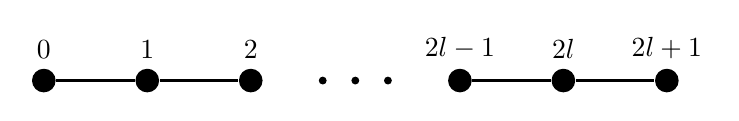
\begin{tikzpicture}[
        node/.style={circle, inner sep=0pt, fill=black, minimum size=3mm},
        node_missing/.style={circle, inner sep=0pt, fill=black, minimum size=1mm}
    ]
    \node[node, label={$0$}] (n1) [] {1};
    \node[node, label={$1$}] (n2) [right=of n1] {2};
    \node[node, label={$2$}] (n3) [right=of n2] {3};
    \node[node_missing] (nm_1) [right=0.7cm of n3] {};
    \node[node_missing] (nm_2) [right=0.3cm of nm_1] {};
    \node[node_missing] (nm_3) [right=0.3cm of nm_2] {};
    \node[node, label={$2l-1$}] (n4) [right=0.7cm of nm_3] {};
    \node[node, label={$2l$}] (n5) [right=of n4] {};
    \node[node, label={$2l+1$}] (n6) [right=of n5] {};
    
    \draw[very thick]  (n1) -- (n2);
    \draw[very thick]  (n2) -- (n3);
    \draw[very thick]  (n4) -- (n5);
    \draw[very thick]  (n5) -- (n6);

    \end{tikzpicture}
    \caption{Illustration, why no Message Passing GNN can detect whether two nodes are in the same connected component. 
    Suppose such a GNN exists and that it has $l$-layers. Consider the graph with $2l+2$ nodes depicted above. 
    Since each node can only share information with its $l$-neighrest neighbors, 
    node 0 can only share information with nodes $0,\cdots,l$
    and node $2l+1$ can only receive information from nodes $l+1,\cdots,2l+1$. 
    Hence, there is no possibility for node $0$ to know about node $2l+1$ and 
    therefore, the GNN cannot detect, whether they are in the same connected component or not.}
    \label{fig:gnn_connectedComponent}
\end{figure}
Besides being impossible to solve this problem with message passing layers, we were asked to present a training process nonetheless. 
The results can be found in figure~\ref{fig:trainingPerc}. 
The model used the settings $d_m, d_u, w_m, w_u$ that were found out do work best in the Bravais class classification as well as the same hyperparameters, 
but with 10 message passing layers instead of just 2 (it seemed reasonable to use a deeper GNN for this task). 
Unsurprisingly, the GNN was not able to solve the percolation problem. 
The accuracy seemingly fluctuates at random between $65\%$ and $75\%$. One might expect to have an accuracy of about $50\%$. 
However, there are graphs which can be fairly easy classified into percolating and non-percolating. 
To give an example, consider a graph that does not have any edge between a node on the left side and a node on the right side of the unit square
(or a node on the bottom and one on the top). By definition, this graph cannot be percolating. 
In this case, the GNN just have to detect, whether such an edge exists or not.
Detecting if such an edge exits is just a matter of measuring lengths of edges, which is easily done,
because each edge is already attributed with its length. 
Furthermore, as the GNN is relatively deep, it is possible, that the network indeed learned to detect percolating graphs, but only when the occurring cycles
have a length that is less than the GNNs depth.
\begin{figure}[h]
    \centering
    \includegraphics[width=0.7\textwidth]{Discussion/plots/percNoPooling.png}
    \caption{Training of a pure message passing GNN on the percolation problem.}
    \label{fig:trainingPerc}
\end{figure}

As we cannot hope to solve the percolation problem with pure message passing layers, 
a natural idea is to try using layers that do not depend on message passing. 
Furthermore, we learned from figure~\ref{fig:gnn_connectedComponent} that the problem lies 
in graphs that are \glqq{}too long\grqq{}, or, putting it differently, that have too many nodes.
Hence, we are looking for layers, that reduce the number of nodes and do not depend on message passing.
That is the reason why we were asked to work with Top-K Pooling layers.
However, there is a good reason, why, even with Top-K Pooling, we cannot hope to achieve 
anything better than in figure~\ref{fig:trainingPerc}.
Recall, that the Top-K Pooling procedure deletes nodes with all its edges and does not create new edges. 
In particular, it does not preserve connected components. To illustrate the point a bit more, 
consider the following situation: Suppose there is a percolating graph $G$. 
After going through the Top-K Pooling layer some nodes might be deleted, 
so that the resulting graph is not percolating anymore. 
Hence, instead of looking at pooling layers that do not respect connected components, we have to look 
at pooling layers, that preserve connected components.
Despite being an interesting challenge, this goes beyond the scope of this project.
However, there are promising approaches and already existing pooling layers, that preserve structures to some extent (for an overview, see for example~\cite{poolingInGNNs}).
Unfortunately, these layers are not yet implemented in PyG and implementing these layers goes well beyond this project.
To conclude, Top-K Pooling layers will not help with the percolation problem. 
Nonetheless, we were again asked to present some training results. We used the same model as above 
with the same hyperparameters but introduced a Top-K Pooling layer after the first message passing layer.
The Top-K Pooling layer was configured so that it reduced the number of nodes by $50\%$.  
The training results can be found in figure~\ref{fig:resTopK}.
At a first sight, the training seems a bit more stable than without the Top-K Pooling layer. 
However, the random fluctuations between $65\%$ and $75\%$ are still present. 
Overall, the training does not show any improvements regarding the accuracy compared to figure~\ref{fig:trainingPerc}.
\begin{figure}[h]
    \centering
    \includegraphics[width=0.7\textwidth]{Discussion/plots/percPooling.png}
    \caption{Training of a message passing GNN additionally equipped with a Top-K Pooling layer on the percolation problem.}
    \label{fig:resTopK}
\end{figure}
 

\section{Conclusion and Outlook}
At this point, we presented all our results and want to reiterate what the 
goals of this project were, which goals we succesfully accomoplished and which 
problems we could not solve.
The primary goal was to get familiar with Graph Neural Networks. 
We succesfully programmed and trained GNNs, understood how message passing works, so that we definitely can say, we took our 
first steps into the GNN-world. Secondly, we wanted build a GNN capable of assigning 2-dimensional and
3-dimensional lattices their Bravais class. We build a GNN that can solve this task with an accuracy of $95\%$, both in 2d and in 3d.
Furthermore, we invastigated the influence of different settings in the message passing procedure. 
The third goal, was to build a GNN than can detect percolation. This problem has not been solved.
We learned, that there are fundamental limitations of GNNs that only rely on message passing.

What can be done next? 
Clearly, for the Bravais classification task one can try to vary node and edge features and try out different training procedures.
However, the more interesting part is probably the percolation problem and related tasks. We already tried to overcome the
limitations of message passing layers with the usage of a TopKPooling layer. However, this layer is not suitable
for the problem at hand. But we have seen that there are layers which might be more suitable. 
Implementing these layers would be a very interesting future challenge.


\printbibliography

\end{document}